\documentclass[a4paper,11pt]{article}
\usepackage[english]{babel}
\usepackage[utf8]{inputenc}
\usepackage{amsmath,amssymb,amsthm,amsfonts}
\usepackage{comment}
\usepackage{fullpage}
\usepackage{xcolor}
\usepackage{url}

%\usepackage[a4paper, total={5in, 8in}]{geometry}



%opening
\title{Lattice-based cryptography}
\author{Damien Stehlé, Adeline Roux-Langlois, Alice Pellet-Mary}

%% Theorems environment
%% Only one counter for all, and depending on the section number
\newtheorem{theorem}{Theorem}[section]
\newtheorem{lemma}[theorem]{Lemma} %% the [theorem] says to use the same counter as for theorem
\newtheorem{properties}[theorem]{Properties}
\newtheorem{proposition}[theorem]{Proposition}
\newtheorem*{remark}{Remark}
\theoremstyle{definition}
\newtheorem{definition}[theorem]{Definition} 
\newtheorem{example}[theorem]{Example}
\newtheorem{exercise}[theorem]{Exercise}
\newtheorem{notations}[theorem]{Notations}

%% To have the table of content appearing on the left
\usepackage{hyperref} 
\setcounter{tocdepth}{2}


\def\labelitemi{$\bullet$}

\newcommand{\mZ}{\mathbb{Z}}
\newcommand{\mR}{\mathbb{R}}
\newcommand{\mQ}{\mathbb{Q}}
\newcommand{\eps}{\varepsilon}
\newcommand{\NN}{\mathbb{N}}
\newcommand{\ZZ}{\mathbb{Z}}
\newcommand{\QQ}{\mathbb{Q}}
\newcommand{\RR}{\mathbb{R}}
\newcommand{\CC}{\mathbb{C}}
\newcommand{\EE}{\mathbb{E}}
\renewcommand{\Pr}{\mathbb{P}}
\newcommand{\Var}{\text{Var}}
\renewcommand{\vec}{\mathbf}
\DeclareMathOperator{\poly}{poly}
\DeclareMathOperator{\adv}{Adv}
\DeclareMathOperator{\dist}{dist}
\renewcommand{\O}{\mathcal{O}}
\newcommand{\Tr}{\mathrm{Tr}}
\newcommand{\N}{\mathcal{N}}
\newcommand{\A}{\mathcal{A}}

\newcommand{\im}{\mathrm{im}}
\renewcommand{\ker}{\mathrm{ker}}

\newcommand{\ps}[2]{\langle#1,#2\rangle}

%%% Alice's macro
\newcommand{\coeff}{\Sigma}
\newcommand{\mink}{\tau}

\begin{document}


\maketitle

Some conventions (?)
\begin{itemize}
\item $n$ the dimension of the lattice
\item bold vectors and matrices (using \texttt{$\setminus$vec})
\item column vectors
\end{itemize}

{\color{red} [Alice: I changed the default setting to have all theorems/lemmas/definitions/... use the same counter. And I made the counter start by the section number. Complain if you prefer something else.]}

\tableofcontents

%!TEX root = main.tex
\section{Lattices}

Dans une partie préliminaire, Damien Stehlé donnera les définitions
élémentaires portant sur les réseaux
euclidiens (bases, minima, volume), qu'il illustrera avec des exemples utiles
pour les
cours avancés (notamment les réseaux $q$-aires). Il abordera les théorèmes
de Minkowski et Minkowski-Hlawka. Ensuite, il introduira
les distributions gaussiennes sur des réseaux,
nécessaires pour les parties suivantes.
%!TEX root = main.tex
\section{LWE, SIS, and cryptographic applications}
\label{se:LBC}

%Dans un deuxième temps, Adeline Roux-Langlois définira les problèmes
%{\emph Learning With Errors} (LWE)
%et {\emph Small Integers Solution} (SIS), qui sont au c{\oe}ur de la
%cryptographie
%reposant sur les réseaux euclidiens. Ensuite, elle décrira les chiffrements
%Primal-Regev et Dual-Regev et prouvera leur sécurité à partir du
%problème LWE. Enfin, elle décrira deux familles de signatures reposant
%sur les réseaux euclidiens, dont sont issus les candidats Dilithium et Falcon
%au processus de standardisation du NIST.


To build cryptographic constructions, we need to rely on problems that are always difficult to solve, as the security of a scheme relies on the hardness of an underlying problem. Ideally, we even have a security proof showing that being able to succeed in an attack breaking the scheme is at least as hard as solving an hard problem.

The SVP or CVP problems may be either very hard to solve, either quite easy, depending on the considered lattice. Then we need to define intermediate problems, which are always difficult to solve.
The Short Integer Solution problem and the Learning With Errors problem are two foundamental problems in lattice(based cryptography, they are used to build many constructions from public key encryption scheme and signature schemes to more advanced schemes.


\subsection{Short Integer Solution problem}

The Short Integer Solution problem (SIS) was introduced by Ajtai in 1996. Intuitively, it asks to find a short vector in the lattice $\Lambda^\perp({\bf A}) = \{ {\bf x} \in \mZ^m: {\bf x}^T \cdot {\bf A} = {\bf 0} \bmod q\}$ previously defined in Definition~\ref{def:qary} for an uniformly random matrix ${\bf A} \in \mZ_q^{n \times m}$, where $q$, $n$ and $m$ are integers such that $m \geq n$.
In 1996, Ajtai also showed that finding a short vector in this particular lattice for an uniform $\bf A$ is at least as hard as solving the GapSVP$_{\gamma}$ problem for an approximation factor $\gamma$ polynomial in the dimension $n$ of the lattice.
This reduction is an worst-case to average-case reduction, meaning that solving a problem for an uniform instance (the average case) is at least as hard as solving a problem for all its instances (including the worst one).


\subsubsection{Gaussian on lattices}

 Gaussian distributions are used in lattice-based cryptography to study the hardness of fundamental problems but also to build constructions. We recall here some basic definitions on Gaussians.
The Gaussian function of center $\mathbf{c} \in \mathbb{R}^{n}$ and width parameter~$\sigma$ is defined as $\rho_{\sigma, \mathbf{c}} (\mathbf{x}) = \exp (- \pi \frac{\left\|\mathbf{x} - \mathbf{c}\right\|^2}{\sigma^2})$, for all $\mathbf{x} \in \mathbb{R}^{n}$. We also define $D_{\sigma,\mathbf{c}}(\mathbf{x}) = \rho_{\sigma,\mathbf{c}}(\mathbf{x}) / \sigma^n$. Gaussians has two nice properties, first they allow to sample short elements (depending of their parameters) with very high probability, we have in particular for $\mathbf{x} \in \mathbb{R}^n$, that $\Pr_{\mathbf{x} \hookleftarrow D_{\sigma}} [\norm{\mathbf{x}} \geq \sqrt{n} \sigma] \leq 2^{-n}$, and second it is easy to add Gaussian as the sum of two Gaussians of parameters $\sigma$ and $\tau$ results in a Gaussian of parameter  ${\sqrt{\sigma^2 + \tau^2}}$. 

The discrete Gaussian distribution over a lattice~$\Lambda$ is obtained by conditioning $D_{\sigma,\mathbf{c}}(\mathbf{x})$ at the event $\mathbf{x} \in \Lambda$, it is defined as $D_{\Lambda, \sigma, \mathbf{c}}(\mathbf{x}) = \frac{D_{\sigma, \mathbf{c}}(\mathbf{x})}{D_{\sigma, \mathbf{c}}(\Lambda)}$, where $D_{\sigma, \mathbf{c}}(\Lambda) = \sum_{\mathbf{x} \in \Lambda} D_{\sigma, \mathbf{c}}(\mathbf{x})$.

Introduced in 2004 by Micciancio and Regev~\cite{MR04}, the \emph{smoothing parameter} of a lattice is an important parameter, which intuitively is the minimum parameter for a discrete gaussian distribution on a lattice to behave like a continuous one (in particular concerning the addition and the size properties). It is formally defined as followed.

\begin{definition}\label{def:smoothing}
For all $\varepsilon >0$, the \emph{smoothing parameter} $\eta_{\varepsilon}(\Lambda)$ of a lattice $\Lambda$ with parameter $\varepsilon$ is defined as the smallest $s$ such $\rho_{1/s}(\Lambda^* \setminus \{0\}) \leq \varepsilon$.
\end{definition}

The size of this parameter is linked to the $n$-th minima of the lattice. In particular, we have~\cite{MR04,Reg05} for any $n$-dimensional lattice $\Lambda$ and $\varepsilon >0$, 
$$\sqrt{\frac{\ln(1/\varepsilon)}{\pi}} \cdot \frac{ \lambda_n (\Lambda)}{n} \leq \eta_{\varepsilon}(\Lambda) \leq \sqrt{\frac{\ln(2n(1+1/\varepsilon))}{\pi}} \cdot \lambda_n (\Lambda). $$

It also allows nice properties on discrete Gaussian on lattices such as a bound on the norm of the sampled elements~\cite{MR04}.
For any $n$-dimensional lattice $\Lambda$, if $s > \eta_{\varepsilon}(\Lambda)$ then
$\Pr_{x \hookleftarrow D_{\Lambda,s,c}} \left[\norm{x-c} > \sqrt{n} s \right] \leq 2^{-n}.$

\begin{lemma}
Let $\Lambda$ and $\Lambda'$ be two lattices of dimension $n$ such that $\Lambda' \subseteq \Lambda$. Then for all $\varepsilon >0$, $s \geq \eta_{\varepsilon}(\Lambda')$ and $\vec{c} \in \mathbb{R}^n$, the distribution $(D_{\Lambda,s,\vec{c}} \bmod \Lambda')$ is at a statistical distance at most $2 \varepsilon$ from the uniform distribution on $(\Lambda \bmod \Lambda')$.
$$ \Delta(D_{\Lambda,s,\vec{c}} \bmod \Lambda', \Lambda \bmod \Lambda') \leq 2 \varepsilon.$$
\end{lemma}

\subsubsection{Definition}

\begin{definition}
\label{def:SIS}
The short integer solution problem (SIS$_{q,m,\beta}$) is as follows: given as input a matrix $\bf A$ uniformly chosen in $\mZ_q^{m \times n}$, the goal is to find~${\bf x} \in \mZ^{m}$ such that ${\bf x}^T {\bf A} =  = 0 \bmod q$ and~$0 < \|{\bf x}\| \leq \beta $. 
\end{definition}

The choice of the parameters $n$, $m$, $q$ and $\beta$ is important to be sure the problem is well defined and difficult to solve. Without the condition on the norm of the vector $\bf x$, this problem is easy to solve, it is equivalent to solve an homogeneous system of linear equation.
It admits a solution for any $q$, ${\bf A} \in \mathbb{Z}_q^{m \times n}$ and $\beta \geq \sqrt{m} q^{n/m}$ (Micciancio Regev 2007).

\begin{figure}[h]
\begin{center}

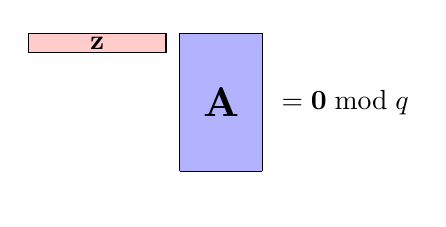
\begin{tikzpicture}[scale=0.35]


\fill[red!20] (-5.5,2.3) rectangle (-0.5,3);
\draw (-5.5,2.3) rectangle (-0.5,3);
\draw (-5.5,2.3) -- (-0.5,2.3);
\draw (-5.5,3) -- (-0.5,3);
\draw (-3,2.65) node {$\bf {z}$};

% Matrice 1
\fill[blue!30] (0,-2) rectangle (3,3) ;
\draw (0,-2) -- (0,3) ;
\draw (3,-2) -- (3,3) ;
\draw (0,-2) -- (3,-2) ;
\draw (0,3) -- (3,3) ;
\draw (1.5,0.5) node[scale=1.5] {$\bf {A}$} ;

\draw (6,0.5) node[scale=1] {$\mathbf{= 0} \bmod q$};

\draw[white] (0,-3) -- (0,-2.8);
\end{tikzpicture} 

\caption{The Short Integer Solution problem.}\label{fig:SIS}
\end{center}
\end{figure}

\paragraph{ISIS.} The ISIS problem is a variant of the SIS problem called the \emph{Inhomogeneous Small Integer Solution} problem. Instead of 
 Au lieu de chercher une solution d'un système homogène, on en cherche une maintenant pour un système d'équations non-homogène.
 
\begin{definition}\label{def:ISIS}
The Inhomogeneous short integer solution problem (SIS$_{q,m,\beta}$) is as follows: given as input a matrix $\bf A$  in $\mZ_q^{m \times n}$, and a vector $\bf{u} \in \mZ_q^n$ both uniformly chosen, the goal is to find~${\bf x} \in \mZ^{m}$ such that~ ${\bf x}^T {\bf A} = {\bf u}^T \bmod q$ and $\|{\bf x}\| \leq \beta $. 

\end{definition}


\subsubsection{Hardness}

In 1996, Ajtai~\cite{Ajtai96} showed that finding a short vector in this particular lattice for an uniform~$\bf A$ is at least as hard as solving the GapSVP$_{\gamma}$ problem for an approximation factor $\gamma$ polynomial in the dimension $n$ of the lattice.
This reduction is an worst-case to average-case reduction, meaning that solving a problem for an uniform instance (the average case) is at least as hard as solving a problem for all its instances (including the worst one). This result is improved in \cite{MR04,GPV08}.



\begin{theorem}[Adapted from~\cite{GPV08}]
\label{th:GPV_SIS}\label{WCAV}
There exists a polynomial time \emph{worst case to average-case} reduction from the \emph{SIVP}$_{\gamma}$ problem to the \emph{SIS}$_{q,m,\beta}$ problem, for any~$m(n), q(n), \beta(n)$ and~$\gamma(n)$ such that $\gamma \geq 2 \beta \sqrt{n}$, $q \geq 2 \beta \sqrt{n}$ and $m,  \log q \leq \text{poly}(n)$.
\end{theorem}


\begin{proof}
We only give the general idea of the proof (and refer to \cite{GPV08} for the full proof), and we simplify it to the case $q = 2 \beta \sqrt{n}$. We also suppose that $\gamma \geq q$ to simplify the reduction, but this condition is not necessary (if $q > \gamma$ we choose $s = \frac{q}{\gamma} \norm{\vec{S}}$).\\


Idea of the reduction: given a basis $\vec{B}$ of a lattice $\Lambda$, we have an oracle which solve SIS, i.e. given a matrix $\vec{A}$ uniform, outputs a short element $\vec{x}$ of norm less than $\beta$ such that  ${\bf x}^T {\bf A} = 0 \bmod q$. The goal is to solve the SIVP problem with an approximation factor $\gamma = 2 \beta \sqrt{n}$.

We use for the reduction a set $\vec{S}$  of linearly independent vectors of the lattice, that we initialize with the basis $\vec{B}$. We then choose a parameter $s =  \norm{\vec{S}} \geq q \cdot  \eta_{\epsilon}(\Lambda)$. 
Note that $\norm{\vec{S}}= \max \norm{\vec{S}_i} \geq \norm{\tilde{\vec{S}}} \geq \eta_{\epsilon}(\Lambda)$, and if $\vec{S}$ is not a solution of SIVP, then $\norm{\vec{S}} \geq \gamma \cdot \lambda_n(\Lambda(\vec{B}))$.\\

The reduction works as follow:
\begin{itemize}
\item Sample $\vec{A}$: for $i=1$ to $m$:
\begin{itemize}
\item $\vec{y}_i \leftarrow D_{\Lambda,s}$ ($\vec{y}_i \in \Lambda$),
\item $\vec{a}_i = \vec{B}^{-1} (\vec{y}_i \bmod q \Lambda) \bmod q \in \mathbb{Z}_q^n$. 
\end{itemize}
We saw that $ \Delta(D_{\Lambda,s,\vec{c}} \bmod \Lambda', U(\Lambda \bmod \Lambda')) \leq 2 \varepsilon$ if $s \geq \eta_{\varepsilon}(\Lambda')$. \\ We have $s \geq q \cdot \eta_{\epsilon}(\Lambda)$ then we have: $ \Delta(D_{\Lambda,s} \bmod q \Lambda, U(\Lambda \bmod q\Lambda)) \leq 2 \varepsilon$ $\Rightarrow$ the $\vec{a}_i$'s are statistically close from uniform in $\mathbb{Z}/ q \mathbb{Z}$. \\
Moreover, the $\vec{y}_i$ 'sare independent, so the $\vec{a}_i$ 'sare too $\Rightarrow$ we can use the SIS oracle.
\item Solving SIS for $\vec{A}$: we obtain nonzero $\vec{z} \in \mathbb{Z}^m$ such that $\vec{z}^T \vec{A} = 0 \bmod q$ and $ 0 < \norm{\vec{z}} \leq \beta$.
\item Combine the elements: let $\vec{x} = \frac{1}{q}\vec{Yz} \in \Lambda$,
\begin{itemize}
\item We first want to show that $\vec{x}$ is an element of the lattice. It suffices to show that $\vec{B}^{-1} \vec{Yz} \in q \mathbb{Z}^m$ (which is equivalent to $\vec{Yz} \in q \Lambda$).  By definition, $\vec{B}^{-1} \vec{Y} = \vec{A} \bmod q$ so $\vec{B}^{-1} \vec{Yz} = \vec{Az} \bmod q = 0 \bmod q$ (it is a solution of the SIS problem).
\item  We have $\norm{\vec{Yz}}  \leq s \beta \sqrt{n}$ then $\norm{\vec{x}} \leq s/2$ $\Rightarrow$ it's a shorter element!
\end{itemize}
To solve SIVP, we repeat this procedure several times to obtain a new set on répète cette procédure plusieurs fois pour obtenir un nouvel ensemble $\vec{S}'$ tel que $\norm{\vec{S}} \leq \norm{\vec{S}'} / 2$. \\
Cette réduction fonctionne aussi pour le problème ISIS en ajoutant un centre bien choisi aux Gaussiennes pour les $\vec{y}_i$.
\end{itemize}
\end{proof}


\subsubsection{Application: hash function}

\begin{definition}
Let $m \geq 4 n \log q$, for a matrix $\vec{A} \in \mathbb{Z}_q^{m \times n}$, we define $f_{\vec{A}} : \{0,1\}^m \rightarrow \mathbb{Z}_q^n$ by:
$$ f_{\vec{A}} (\vec{x}) = \vec{x}^T \vec{A} \bmod q.$$
\end{definition}


We start with an important lemma, which shows that for any input $\vec{x}$, the output $ \vec{x}^T \vec{A}$ is statistically indistinguishable from a uniform element in $\mZ_q^{n}$, knowing $\vec{A}$. It is called a Leftover Hash Lemma.

\begin{lemma}
\label{le:LHL}
Let $m, n, q \ge 1$ be integers such that $m \geq 4 n \log q$ and $q$ is prime, and let $\vec{A} \hookleftarrow U(\mZ_q^{m \times n})$ and $\vec{r} \hookleftarrow U(\{0,1\}^m)$. Then the statistical distance between $(\vec{A},\vec{r}^T \vec{A})$ and the uniform distribution on $\mZ_q^{m \times n} \times \mZ_q^{n}$ is less than $\leq 2^{-n}$.
\end{lemma}

The condition  $m \geq 4 n \log q$ is important, it allows sufficient entropy.



\begin{theorem}
\label{th:resistanceCollision}
If the SIS problem is difficult to solve for $\beta \geq \sqrt{m}$, then the Ajtai's hash function is collision resistant.
\end{theorem}

\subsection{Learning With Errors problem}

The LWE problem was introduced by Regev in 2005~\cite{Reg05}. Intuitively, it asks to solve a BDD instance (see Definition~\ref{def:BDD}) in the following lattice $ \Lambda_q(\vec{A}) = \{ \vec{y} \in \mathbb{Z}^m : \vec{y} =\vec{As} \bmod q \text{ for } \vec{s} \in \mathbb{Z}^n\},$ previously defined in Definition~\ref{def:qary} for an uniformly random matrix ${\bf A} \in \mZ_q^{n \times m}$, where $q$, $n$ and $m$ are integers such that $m \geq n$.




\subsubsection{Definition}

The computational variant of LWE asks to find a vector $\vec{s} \in \mZ_q^n$ given an arbitrary number of noisy scalar product between $\vec{s}$ and some known $\vec{a}_i$'s uniformly chosen in $\mZ_q^n$. Its decisional variant asks to distinguish those noisy scalar products from uniform elements.

\begin{definition}
Let $n \geq 1$, $q\geq 2$ prime, and $\alpha \in ]0,1[$. The distribution $D^{\mbox{\tiny LWE}}_{n,q,\alpha}(\vec{s})$ is a distribution on
$\mZ_q^{n+1}$ obtained with the following experiment: 
\begin{itemize}
\item sample $\vec{a} \hookleftarrow U(\mZ_q^n)$,
\item sample $e \hookleftarrow D_{\mZ,\alpha q}$,
\item Output $(\vec{a}, \ps{\vec{a}}{\vec{s}} +  e \bmod q )$.
\end{itemize}
The Learning with Errors problem is defined as follow:
\begin{itemize}
\item Search variant of LWE$_{n,q,\alpha}$: Let $\vec{s} \leftarrow U(\mZ_q^{n})$, given an arbitrary number of samples from $D^{\mbox{\tiny LWE}}_{n,q,\alpha}(\vec{s})$, find $\vec{s}$.
\item Decisional variant of LWE$_{n,q,\alpha}$: Let $\vec{s}\hookleftarrow U(\mZ_q^{n})$,  distinguish between the distributions $D^{\mbox{\tiny LWE}}_{n,q,\alpha}(\vec{s})$ and $U(\mZ_q^{n} \times \mZ_q)$.
\end{itemize}
\end{definition}

Usually, the parameter $q$ is chosen polynomial in $n$ and $\alpha$ is chosen between $1/q$ and $q$.
The choice of $\alpha$ is important here, if it is too small, the noise of each sample can be zero with high probability and then it is easy to find $\vec{s}$. If $\alpha$ is too large, then $e$ can be close to be uniformly distributed modulo~$q$. The distribution $D^{\mbox{\tiny LWE}}_{n,q,\alpha}(\vec{s})$ will be too close from uniform and independant from $\vec{s}$ and then it will be impossible to find $\vec{s}$.




\subsubsection{Reduction from search to decision}

Regev~\cite{Reg05} showed an important result on the equivalence of the two version of LWE.

\begin{lemma}
The two LWE variants, search and decisional, are computationally equivalent.
\end{lemma}

It is an interesting property as search problems are usually harder than decision ones, but in security proofs we often rely on a decisional problem. The first direction of the reduction is quite direct since if we are able to solve the search problem, the resulting secret would allow to distinguish between an LWE distribution and a uniform one.


\begin{proof}
Suppose that an algorithm $\mathcal{A}$ can efficiently solve the decisional variant of LWE, we will use it to solve the search variant.
We start by solving this variant with a non negligible probability on $\vec{s} \hookleftarrow U(\mZ_q^n)$. 
We have access to an oracle sampling from $D^{\mbox{\tiny LWE}}_{n,q,\alpha}(\vec{s})$, and to $\mathcal{A}$, 
and we want to find $\vec{s}$. Let's show how to find the first coordinate $s_1$ 
of~$\vec{s}$. As $q$ is small, one can try all the possible values $s_1^*$ of~$s_1$, and then use~$\mathcal{A}$ to validate this value. Using a sample $(\vec{a},b)= (\vec{a}, \ps{\vec{a}}{\vec{s}} + e)$, 
we give to $\mathcal{A}$ the following input 
\[(\vec{a},b)+ (u,0,\ldots,0, u s_1^*) = (\vec{a}', \ps{\vec{a}'}{\vec{s}} + e + u (s_1^*-s_1)), \ 
\mbox{avec} \ u \hookleftarrow U(\mZ_q).
\]
Then:
\begin{itemize}
\item if $s_1^* = s_1$, the input sample given to $\mathcal{A}$ is following the
$D^{\mbox{\tiny LWE}}_{n,q,\alpha}(\vec{s})$ distribution;
\item if $s_1^* \neq  s_1$, then the last coordinate is uniformly distributed and independent from the $n$ other, as $u$ is uniform and $s_1^*-s_1$ invertible modulo~$q$.
\end{itemize}   
The answer of $\mathcal{A}$ tells us if the guess~$s_1$ for is correct.

If it is possible to find $\vec{s}$ with a non-negligible probability, when $\vec{s} \hookleftarrow U(\mZ_q^n)$, then it is possible for any $\vec{s}$.
Indeed, for a fixed $\vec{s}$, we can sample $\vec{t} \hookleftarrow U(\mZ_q^{n})$, and transform the sample $(\vec{a},\ps{\vec{a}}{\vec{s}} + e)$ of $D^{\mbox{\tiny LWE}}_{n,q,\alpha}(\vec{s})$ in a sample $(\vec{a},\ps{\vec{a}}{\vec{s} + \vec{t}} + e)$ of $D^{\mbox{\tiny LWE}}_{n,q,\alpha}(\vec{s}+\vec{t})$.
As $\vec{s}+\vec{t}$ is uniform, we can find $\vec{s}+\vec{t}$, and then~$\vec{s}$.
\end{proof}

This first reduction is provided only for~$q$ prime and $\text{poly}(n)$, but for any error distribution. It also needs $m' = \tilde{O}(nmq/\varepsilon^2)$ search LWE samples to call the decision oracle with $m$ samples, where $\varepsilon$ is the advantage of the oracle to distinguish between the two distributions. 
The conditions on the parameters of this reduction (in particular on $q$) was later improved in several works~\cite{Pei09,MP12,BLPRS13}, but only for Gaussian distributions, and with a similar loss on the number of samples.
There also exists a sample-preserving search-to-decision reduction given by Micciancio and Mol~\cite{MM11}, this reduction only works for particular cases, as for instance $q$ prime and $\text{poly}(n)$ for any discrete error on $\mZ_q$.


\subsubsection{Hardness of LWE}



\paragraph{Quantum reduction.} Regev~\cite{Reg05,Reg09} was the first to provide a worst-case to average-case reduction showing the hardness of the Learning With Errors problem. This reduction has the particularity to use a quantum algorithm. This mean given an oracle to solve LWE, we only have a quantum algorithm to solve Approx-GapSVP. Then, if it happens that an attacker can solve LWE, he will need a quantum computer to polynomially solve Approx-GapSVP or SIVP for all possible instances (i.e. even in the worst-case). 

\begin{theorem}[{\cite[Th. 1.1]{Reg05}}]
Let $q >2$ and $\alpha \in (0,1)$ be function of $n$ such that $\alpha q \geq 2 \sqrt{n}$. If $q$ is prime and polynomial in $n$, then there exists a worst-case to average-case quantum polynomial time reduction from \emph{GapSVP}$_{\gamma}$ (or \emph{SIVP}$_{\gamma}$) in dimension~$n$ to \emph{LWE}$_{n,q,\alpha}$ for $\gamma = \tilde{O}(n/\alpha)$. 
\end{theorem}


\paragraph{High level idea of Regev's proof.} We refer to~\cite{Reg05} for the full proof. 
Regev defines an intermediate problem called DGS (discrete Gaussian sampling problem):


\begin{itemize}
\item DGS$_{\phi}$: given a lattice $\Lambda$ of dimension $n$ and a parameter $r > \phi(\Lambda)$. Output a sample of $D_{\Lambda,r}$.
\end{itemize}
Remark: the hardness of this problem depends on the basis of $\Lambda$ that we have. Then the smaller is $r$, the harder it is to solve.
Then Regev described two reductions:

\medskip

%\lecours{\textcolor{blue}{

\begin{itemize}
\item A reduction from SIVP with $\gamma=\tilde{O}(n / \alpha)$ to DGS with $r=2 \sqrt{n} \eta_{\varepsilon}(\Lambda) / \alpha$.
\begin{itemize}
\item Principle of the reduction from SIVP$_{2\sqrt{n} \phi(L)}$ to DGS$_{\phi(L)}$ if $\phi(L) \geq 2  \eta_{\varepsilon}(L)$:
\begin{itemize}
\item Given a lattice $L$, we start by using LLL to obtain $S$ = set of $n$ vectors linearly independent of size at most $2^n \lambda_n(L)$. We denote by $\tilde{\lambda}_n$ the norm of the largest, by construction $\lambda_n(L) \leq \tilde{\lambda}_n \leq 2^n \lambda_n(L) $.
\item For $i \in \{0, \ldots, 2n \}$, call DGS $n^2$ times on $(L,r_i = \tilde{\lambda}_n 2^{-i})$ to build the set $S_i$. (check if $r_i > \phi(L)$)
\item Choose the $n$ vectors linéairement linearly independent in each $S_i$ and output the shortest set.
\end{itemize}
\item Why does it work?
\begin{itemize}
\item If $\phi(L) \geq \tilde{\lambda}_n $, $S$ is already smaller than $2 \sqrt{n} \phi(L)$.
\item Else, let $i$ such that $\phi(L) < r_i < 2 \phi (L)$ (exists because $\lambda_n(L) \leq \tilde{\lambda}_n \leq 2^n \lambda_n(L) $, $\phi(L) \geq 2  \eta_{\varepsilon}(L)$ and $\eta_{\varepsilon}(L) \geq \lambda_n(L)/n$). There are  $n$ vectors linearly independent in $S_i$ with high probability (see Corollary 3.16 Regev 09). All the vectors of $S_i$ has norm at most $\sqrt{n} r_i \leq 2 \sqrt{n} \phi (L)$.
\end{itemize}
\end{itemize}
\item If $\alpha q > 2 \sqrt{n}$, a quantum reduction from DGS for $r= \sqrt{2n} \eta_{\varepsilon}(\Lambda) / \alpha$ to LWE$_{q,\alpha}$.
\begin{itemize}
\item Input : a lattice $L$ and $r > 2 \sqrt{n} \eta_{\varepsilon}(\Lambda) / \alpha$. Goal: a sample from $D_{L,r}$.
\item Principle: two iterations. Let $r_i = r \cdot (\alpha q / \sqrt{n})^i$. The algorithm starts by producing $n^c$ samples of $D_{L,r_{3n}} $ (he can do it because $r_{3n} > 2^{3n}r > 2^{2n} \lambda_n(L)$). Iteration:
\begin{itemize}
\item Classical step: given $n^c$ samples of $D_{L,r_i}$ and an LWE oracle, solve CVP$_{L^*,\frac{\alpha q}{r}}$ (variant where the distance between the target and the lattice is $\frac{\alpha q}{r}$). 
\item Quantum step: use the CVP$_{L^*,\frac{\alpha q}{r}}$ oracle to find $n^c$ samples of $D_{L,r_{i-1}}$.
\end{itemize}
\item At the end, we have $n^c$ samples of $D_{L,r_0}$ with $r_0=r$.
%$r_ 1 =r \cdot \alpha q / \sqrt{n} > \sqrt{2} q \eta_{\varepsilon}(\Lambda) $
\end{itemize}
\end{itemize}
%}


\paragraph{Classical reductions.} In 2009, Peikert~\cite{Pei09} gave the first classical reduction to show the hardness of the LWE problem, but his result was limited to an exponential modulus $q$ in the dimension $n$. Compared to the original reduction of Regev, this reduction is also limited to GapSVP.

\begin{theorem}[{\cite[Th. 3.1]{Pei09}}]
Let $q >2$ and $\alpha \in (0,1)$ be function of $n$, there exists a worst-case to average-case classical polynomial time reduction from \emph{GapSVP}$_{\gamma}$ in dimension~$n$ to \emph{LWE}$_{n,q,\alpha}$ for $\gamma \geq \frac{n}{\alpha \log n}$ and $q \geq 2^{n/2} \cdot \omega(\sqrt{\log n /n})$. 
\end{theorem}

\paragraph{Classical hardness for a polynomial modulus.} In 2013~\cite{BLPRS13}, Brakerski \emph{et al.} provided a classical reduction to show the hardness of the Learning With Errors problem, for a polynomial modulus $q$ in the dimension $n$. This smaller size of the modulus is the one used in practice, this reduction also remove the condition on~$q$ to be prime.

\begin{theorem}[{\cite{BLPRS13}}]
Let $q >2$ and $\alpha \in (0,1)$ be function of $n$ such that $\alpha q \geq \sqrt{n}$. There exists a worst-case to average-case classical polynomial time reduction from \emph{GapSVP}$_{\gamma}$ in dimension~$\sqrt{n}$ to \emph{LWE}$_{n,q,\alpha}$ for $\gamma = \tilde{O}(n^2/\alpha)$. 
\end{theorem}

The main idea of this reduction is to start from Peikert's result, i.e. a classical reduction from GapSVP to LWE for an exponential modulus. And then to use a modulus switching technique to provide a reduction from LWE with an exponential modulus to LWE with a polynomial modulus, at the expense of making the error term grows. 
 Note than an important step for this reduction to work is to use LWE with a smaller secret.
Overall, this reduction looses a factor $\sqrt{n}$ in the dimension of the two problems, if we compare to Regev's quantum reduction.
Those results can be summarised in Table~\ref{tab:LWE}.

\begin{table}[h]
\begin{center}
\begin{tabular}{c|c|c|c|c|c}
%\hline
& dim $n'$ & $q$ & $\alpha$ & $\gamma$ & \\
\hline
\cite{Reg05} & $n$ & $\text{poly}(n)$, prime  & $\alpha q \geq 2\sqrt{n}$& $\tilde{O}(n/\alpha)$ & quantum \\[0.3em]
\cite{Pei09} & $n$ & $q> 2^{n/2}$ & $\alpha q \geq n$ & $ \geq n /(\alpha \log n)$ & classical \\[0.3em]
\cite{BLPRS13} & $\sqrt{n}$ & $\text{poly}(n)$ & $\alpha q \geq \sqrt{n}$ & $\tilde{O}(n^2/\alpha)$ & classical \\
%\hline
\end{tabular}
\caption{Reductions from GapSVP$_{n', \gamma}$ to LWE$_{n,q,\alpha}$.}
\label{tab:LWE}
\end{center}
\end{table}

Finally, an important consequence of the work of~\cite{BLPRS13} is to show that the hardness of LWE in dimension $n$ and with a modulus $q$ is a function of $n \log q$. This is shown by the modulus switching reduction which gives a reduction from LWE$_{n,q}$ to LWE$_{n/k,q^k}$ and from LWE$_{n,q^k}$ to LWE$_{nk,q}$.





\paragraph{Other variants.}
In the original LWE problem, the secret is uniformly sampled in $\mZ_q^n$. But there are other possible distributions for the secret, which were introduced in several articles for different cryptographic applications.

\begin{itemize}
\item In 2009, the first result~\cite{ACPS09} by Applebaum, Cash, Peikert and Sahai showed that the secret could have the same distribution as the error. In particular, for $q$ a prime power, they provided a polynomial-time reduction from LWE$_{n,q,\chi}(U(\mZ_q^n))$ to LWE$_{n,q,\chi}(\chi^n)$. As a consequence, the LWE problem with both secret and error following a discrete Gaussian distribution can also be considered as a hard problem, and is usually called HNF-LWE. This reduction was extended to any $q$ in~\cite{BLPRS13}.
\item In 2010, Goldwasser, Kalai, Peikert and Vaikuntanathan~\cite{GKPV10} studied the robustness of the Learning With Errors assumption by considering leaky secrets. They considered that the secret follows a distribution $\mathcal{D}$ with min-entropy $k$, and showed that there exists a polynomial time reduction from LWE$_{\ell,q,\alpha}(U(\mZ_q^n))$ to LWE$_{n,q,\beta}(\mathcal{D})$ for $k \geq \ell \log q + \omega( \log n)$ and $\alpha / \beta = \text{negl}(n)$. The main drawback of their result is this last condition on the parameters, which comes from a noise flooding argument in the reduction, as $\beta$ needs to be very large to satisfy it. This gives in particular the first reduction to show the hardness of the binary variant of LWE, called bin-LWE, where the secret is sampled uniformly in~$\{0,1\}^n$. This result is improved in~\cite{BLPRS13}. The high level idea of the reduction is similar to the one in~\cite{GKPV10}, but to avoid the last argument using noise flooding, the author used and proved the hardness of the extended-LWE problem. The principle of this new problem is to give an additional information on the noise of the LWE samples. This allows to achieve a reduction from LWE$_{\ell,q,\alpha}$ to bin-LWE$_{n,q,\beta}$ for $n \geq \ell \log q + \omega( \log n)$ and $\alpha / \beta = 1 / \sqrt{10n}$.
In 2018, Micciancio~\cite{Mic18} proposed a much simpler reduction to prove the hardness of LWE with binary secret, with a similar conditions on the parameters, i.e. $\alpha / \beta = 1 / (2 \sqrt{n+1})$.
\item Recently, Brakerski and Döttling~\cite{BD20} extended the hardness of LWE to more general secret distribution. They showed that the hardness depends directly on a property of the distribution of the secret that they call the noise lossiness. One difference with the previous results is that they loose a factor $\sqrt{m}$, where $m$ is the number of samples, between the Gaussian parameters.
\end{itemize}
The original quantum reduction of Regev~\cite{Reg05} and the two classical reductions~\cite{Pei09,BLPRS13} all use a continuous gaussian distribution for the error term of the LWE sample. 
The distribution defined by Regev is a distribution on $\mathbb{T}$ called $\psi_{\beta}$ for a parameter $\beta \in \mathbb{R}^+$, which is obtained by sampling from a normal variable with standard deviation $\beta / \sqrt{2 \pi}$ and reducing the result modulo $1$. Regev also showed in~\cite[Lemma 4.3]{Reg05} that the problem is still hard using a discretization of the probability density function for the error on $\mZ_q$ (and in particular in the case of rounded Gaussian).

Discrete Gaussian directly sampled from $D_{\mZ,\alpha q}$ for $\alpha \in [0,1)$ is a popular distribution for the error for many of the applications. The reduction from LWE with a continuous Gaussian distribution to LWE with a discrete one is formalized by Peikert's result~\cite{Pei10} using Theorem~3.1.
This article also proposes an efficient sampler for discrete Gaussian distributions over a lattice. However building efficient and secure Gaussian samplers appear to be a complicated task, and recent results show that it is possible to use side-channel attacks against existing samplers~\cite{BHLY16,Pessl16,Saarinen18}. 
An other drawback of Gaussian distributions is that the existing sampler are not exacts ones, then provide different distributions than the exact one used in the reduction. 
Then, and mainly for practical reasons, other distributions were studied for the error term of~LWE.
\begin{itemize}
\item  The LWE problem with noise uniform in a small interval $[-\beta,\beta]$ was first introduced by Döttling and Müller-Quade~\cite{DMQ13}. The authors exhibit a reduction from LWE with Gaussian noise. The main proof ingredients are the construction of lossy codes for LWE (which are lossy for the uniform distribution in a small interval), and the fact that lossy codes are pseudorandom. The reduction from~\cite{DMQ13} needs the number of LWE samples to be fixed and bounded by poly$(n)$, and $\beta \geq m n^c \alpha$ where  $\alpha$ is the LWE Gaussian noise parameter and $c \in (0,1)$ is an arbitrarily small constant. Note that it also degrades the LWE dimension by a constant factor, but that there is no condition on $q$. 

The LWE problem with uniform noise in a small interval is also investigated in~\cite{MP13}, with a focus on the number of LWE samples. The reduction from~\cite{MP13} does not preserve the LWE dimension either.
Another reduction~\cite{BGMRR16} for LWE with uniform noise can be obtained by using the hardness result for the Learning With Rounding (LWR) problem~\cite{BPR12}. The resulting reduction maps the LWE$_{n',q,\alpha,m}$ problem to the LWE$_{n,q,U([-\beta,\beta]),m}$ problem with $n'=n/\log q $ and $\beta= \Omega(m \alpha/\sqrt{\log n})$. 

An alternative proof is provided in~\cite{BLLSS15}, which is marginally more general as it also applies to distributions with smaller noises.
Moreover, this reduction preserves the dimension~$n$ of LWE, and is hence tighter than the one from~\cite{DMQ13} (which degrades the LWE dimension by a constant factor).
\item The particular case of a binary noise is introduced in~\cite{MP13}. Micciancio and Peikert showed the hardness of this problem, by providing a reduction from LWE, but with a bounded number of samples $m=n \cdot (1+ \Omega(1/ \log n))$. Indeed, the problem becomes insecure for more samples, in particular using Arora-Ge attack as studied in~\cite{AG11,BGPW16}.
\end{itemize}




\subsection{Public Key encryption scheme on LWE}


Note: la partie qui suit sera traduite en anglais dans la version finale.


\subsubsection{Regev's encryption scheme}

Le premier chiffrement dont la sécurité repose sur la difficulté du problème LWE a été proposé par Regev en 2005. La dimension $n$ est le paramètre de sécurité de ce chiffrement. Les autres paramètres sont $m$, $q$ et $\alpha$. Dans la description qui suit, toutes les opérations se font modulo l'entier~$q$.

Le principe de ce chiffrement est de donner comme clé publique des échantillons $(\vec{a}_i,b_i)$ de la distribution $D_{n,q,\alpha}^{\mbox{\tiny LWE}}(\vec{s})$, et de conserver comme clé secrète le vecteur~$\vec{s}$.
Pour chiffrer un clair $M \in \{0,1 \}$, on choisit un vecteur $\vec{r}$ uniformément dans $\{0,1 \}^m$, 
ce qui correspond à choisir un sous-ensemble aléatoire des couples $(\vec{a}_i,b_i)$. 
On fait ensuite la somme les couples choisis, puis on ajoute $\lfloor q/2 \rfloor \cdot M$ à la somme des~$b_i$.
Pour déchiffrer un chiffré $(\vec{u}^T,v)$ correctement généré, on utilise la clé secrète~$\vec{s}$ pour 
calculer $v - \vec{u}^T \vec{s} =  \vec{r}^T \vec{e} + \lfloor q/2 \rfloor \cdot M $. Or le vecteur $\vec{e}$ est échantillonné selon une gaussienne discrète de paramètre 
$\alpha q \leq q/(4m)$, ainsi $\vec{r}^T \vec{e}$ est petit par rapport à $q/2$.
La valeur de $v - \vec{u}^T \vec{s}$ est donc soit proche de~$0$, soit proche de $\lfloor q/2 \rfloor$, ce qui permet de 
retrouver le clair~$M$.


\begin{definition}[Chiffrement de Regev] 
Soient $n$, $m$, et $q$ des entiers avec $q$ premier et $m \geq 4 (n+1) \log_2 q$, 
et $\alpha$ un réel dans~$]0,1/(8m)[$.

\begin{description}
\item[$\mathsf{KeyGen}$ :]
La clé secrète est $\vec{s} \hookleftarrow U (\mZ_q^n)$. La clé publique est un couple $(\vec{A}, \vec{b}) = (\vec{A}, \vec{As} + \vec{e})$, où $\vec{A} \hookleftarrow U (\mZ_q^{m \times n})$ et 
$\vec{e} \hookleftarrow D_{\mZ^m, \alpha q}$. 

\item[$\mathsf{Enc}$ :]
\'Etant donné $M \in \{0,1 \}$, échantillonner $\vec{r} \hookleftarrow U(\{0,1 \}^m)$ et renvoyer le chiffré $$( \vec{r}^T \vec{A}, \vec{r}^T \vec{b} + \lfloor q/2 \rfloor \cdot M)
\in \mZ_q^{n} \times \mZ_q.$$

\item[$\mathsf{Dec} $ :] 
\'Etant donné un chiffré $(\vec{u}^T,v) \in \mZ_q^{n} \times \mZ_q$, calculer $v - \vec{u}^T \vec{s}$: le clair est $0$ si le résultat est plus proche de $0$ que de $\lfloor q/2 \rfloor$, 
et $1$ sinon.
\end{description}
\end{definition}


Remarque : la fonction de chiffrement ne permet de chiffrer qu'un seul bit. Pour en chiffrer plusieurs, on peut soit l'utiliser plusieurs fois, soit utiliser plusieurs colonnes $\vec{b}_j$ au lieu d'une seule.

\paragraph{Correction.}
Le vecteur $\vec{r}$ est choisi uniformément dans $\{0,1 \}^m$, 
et le vecteur $\vec{e}$ est échantillonné selon une gaussienne discrète de paramètre 
$\alpha q \leq q/(8m)$, ainsi, nous savons qu'avec probabilité proche de~1, 
\[ 
\big| \sum_{i \leq m} r_i e_i \big| \leq \|\vec{r}\| \cdot \|\vec{e}\| \leq \sqrt{m} \cdot \frac{q}{8\sqrt{m}} = \frac{q}{8}.
\]
La valeur de $v - \vec{u}^T \vec{s}$ est donc soit proche de~$0$, soit proche de $\lfloor q/2 \rfloor$, ce qui permet de 
retrouver le clair~$M$.

\paragraph{Sécurité.}

\begin{theorem}
Le chiffrement de Regev est IND-CPA sous l'hypothèse que LWE est difficile. 
\end{theorem}


\subsubsection{Dual Regev encryption scheme}

En 2008, Gentry, Peikert et Vaikuntanathan ont proposé un autre chiffrement, appelé \emph{dual-Regev}. Le principe du chiffrement de Dual-Regev est de donner comme clé publique $\vec{y}^T = \vec{r}^T \vec{A}  \bmod q$ et de garder comme clé secrète le vecteur~$\vec{r}$.

On utilise ensuite LWE pour chiffrer le message: on prend un $\vec{s}$ uniforme, et le chiffré $(\vec{b},c)$ correspond à $m+1$ membres droits d'échantillons, avec les lignes de $\vec{A}$ 
et le vecteur $\vec{y}$ comme membres gauches. Pour déchiffrer $(\vec{b},c)$, il suffit de calculer:
\[
c - \vec{r}^T \vec{b} = \vec{y}^T \vec{s} + e' + \lfloor q/2 \rfloor \cdot M - \vec{r}^T (\vec{A} \vec{s} + \vec{e} ) 
= e'-\vec{r}^T \vec{e} + \lfloor q/2 \rfloor \cdot M.
\]
Comme pour le chiffrement de Regev, le paramètre $\alpha$ a été choisi pour que $e'-\vec{r}^T \vec{e}$ soit petit devant~$q/2$, ainsi, la valeur de $c - \vec{r}^T \vec{b}$ 
permet de retrouver~$M$.


\begin{definition}[Chiffrement dual-Regev] 
Soient $n$, $m$, et $q$ des entiers avec $q$ premier et $m \geq 4 n  \log_2 q$, 
et $\alpha$ un réel dans~$]0,1/(16m)[$. Les utilisateurs partagent une matrice $\vec{A} \hookleftarrow U(\mZ_q^{m\times n})$.

\begin{description}
\item[$\mathsf{KeyGen}$ :]
La clé secrète est $\vec{r} \hookleftarrow U(\{0,1\}^m)$. La clé publique est $\vec{y}^T =  \vec{r}^T \vec{A} \bmod q$.

\item[$\mathsf{Enc}$ :]
\'Etant donné $M \in \{0,1 \}$, échantillonner $\vec{s} \hookleftarrow U (\mZ_q^n)$, $\vec{e} \hookleftarrow D_{\mZ^m, \alpha q}$ et 
$e' \hookleftarrow D_{\mZ, \alpha q}$. Le chiffré est $$(\vec{A}\vec{s}+\vec{e},\vec{y}^T \vec{s} + e' + \lfloor q/2 \rfloor \cdot M) \in \mZ_q^{m} \times \mZ_q.$$

\item[$\mathsf{Dec}$ :] 
Etant donné un chiffré $(\vec{b},c)$, calculer $c - \vec{r}^T \vec{b}$: le clair est $0$ si le résultat est plus proche de $0$ que de $\lfloor q/2 \rfloor$, et $1$ sinon.

\end{description}
\end{definition}

\paragraph{Correction.}
Pour déchiffrer $(\vec{b},c)$, il suffit de calculer:
\[
c - \vec{r}^T \vec{b} = \vec{y}^T \vec{s} + e' + \lfloor q/2 \rfloor \cdot M - \vec{r}^T (\vec{A} \vec{s} + \vec{e} ) 
= e'-\vec{r}^T \vec{e} + \lfloor q/2 \rfloor \cdot M.
\]

Le vecteur $\vec{r}$ est choisi uniformément dans $\{0,1 \}^m$, 
le vecteur $\vec{e}$ est échantillonné selon une gaussienne discrète de paramètre $\alpha q \leq q/(16m)$, et l'élément $e$ est aussi échantillonné selon une gaussienne discrète de paramètre $\alpha q$, ainsi, nous savons qu'avec probabilité proche de~1, 
\[ 
\big| e' - \sum_{i \leq m} r_i e_i \big| \leq |e'| + \|\vec{r}\| \cdot \|\vec{e}\| \leq  \sqrt{m} \cdot \alpha q + \sqrt{m} \cdot \sqrt{m} \alpha q \leq 2 \sqrt{m} \frac{q}{16\sqrt{m}} = \frac{q}{8}.
\]
La valeur de $v - \vec{u}^T \vec{s}$ est donc soit proche de~$0$, soit proche de $\lfloor q/2 \rfloor$, ce qui permet de 
retrouver le clair~$M$.

\medskip





\paragraph{Sécurité.} 

\begin{theorem}
Le chiffrement de Dual-Regev est IND-CPA sous l'hypothèse que LWE est difficile. 
\end{theorem}

\begin{proof}
Le schéma de chiffrement dual-Regev est IND-CPA. 
Les arguments de sécurité sont les mêmes que pour le schéma de chiffrement de Regev, mais utilisés dans un ordre différent.\\
Le \emph{leftover hash lemma} garantit que la distribution des données publiques $(\vec{A},\vec{y})$ est essentiellement uniforme.
Ainsi, le masque $(\vec{A}\vec{s}+\vec{e},\vec{y}^T \vec{s} + e')$ utilisé dans la procédure de chiffrement 
est essentiellement distribué comme $m+1$ échantillons de la distribution $D_{n,q,\alpha}^{\mbox{\tiny LWE}}(\vec{s})$ (pour un vecteur $\vec{s} \hookleftarrow U(\mZ_q^n)$).\\
\'Etant donné un chiffré $(\vec{b},c)$, la  distribution de  $(\vec{A},\vec{b},\vec{y},c)$ est calculatoirement indistinguable de la distribution uniforme, sous 
l'hypothèse que le problème LWE est difficile.
\end{proof}

\paragraph{Remarque.} Les deux schémas de chiffrement décrits sont IND-CPA mais ne sont pas IND-CCA. Il existe cependant plusieurs schémas de chiffrement qui sont IND-CCA sous l'hypothèse que LWE est difficile.

\subsection{Signature scheme}



\subsubsection{Signature using Fiat Shamir transformation}

Les signatures dites de type "Fiat-Shamir" sont construites à partir d'un schéma d'identification. Un schéma d'identification est un protocole en 3 passes : Commitment, Challenge, Réponse, qui permet à un \emph{Prouveur} (possédant une clé secrète) de prouver son identité à un \emph{Vérifieur} (qui possède la clé publique associée).

\begin{center}
\begin{tabular}{c  c  c}
 Prouveur$_{sk}$ & &  Vérifieur$_{pk}$ \\
\hline \\
& $\overset{CMT}{\rightarrow}$ & \\
& $\overset{CH}{\leftarrow}$ & $CH \leftarrow U(\{0,1\}^{\lambda})$ \\
& $\overset{RSP}{\rightarrow}$ & Etant donné $ CMT || CH || RSP$ \\
&  & Accepte ou non \\
\hline
\end{tabular} \end{center}

\bigskip

En 1986, Fiat et Shamir ont proposé une transformation qui permet de construire un schéma de signature à partir d'un schéma d'identification dans le modèle de l'oracle aléatoire. Le principe est le suivant : l'algorithme de signature est en fait ce qu'exécute le \emph{Prouveur}, en choisissant lui même le challenge $CH$ à partir d'une fonction de hachage $H$ : $CH \leftarrow H(CMT,m)$. La signature d'un message $m$ est ensuite $\sigma = (CMT, RSP)$ et pour vérifier une signature de ce type, il suffit de calculer le challenge $CH = H(CMT,m)$ et de vérifier que $ CMT || CH || RSP$ est valide.

La sécurité de la signature repose ensuite directement sur la sécurité du schéma d'identification, et est nécessairement dans le modèle de l'oracle aléatoire. %L'avantage ici par rapport au schéma précédent est qu'il n'y a plus besoin d'utiliser de trappe.


%\paragraph{Construction sur les Réseaux.}
%Décrivons maintenant la construction de Lyubashevsky 2012.

\begin{figure}[!h]
\rule{\linewidth}{.5pt}
%\begin{definition}[GPV signature] 
Soient $k=80$, $n, m$ et $q$ des entiers, et soit~$s$ un paramètre gaussien. Choisir une fonction de hachage $\mathcal{H} : \{0, 1\}^* \rightarrow \{ -1,0, 1\}^k$ qui peut être modélisée comme un oracle aléatoire.
\vspace*{-0.2cm}
\begin{description}
\item[$\mathsf{KeyGen}(k,n,m,q) \rightarrow (vk,sk)$.] \'Etant donnés les paramètres,
générer une matrice $\vec{S} \in \{-1,0,1 \}^{k \times m}$ uniforme et une matrice $\vec{A} \in \mZ_q^{m \times n}$ uniforme, puis calculer $\vec{T}=\vec{SA} \bmod q$. 
\begin{itemize}
\item \textbf{Clé de vérification} : $pk = (\vec{A}, \vec{T})$.
\item \textbf{Clé secrète} : $sk = \vec{S}$.
\end{itemize}

\item[$\mathsf{Sign}(k,n,m,sk,M \in \{0,1\}^{*}) \rightarrow \vec{v} $.] \'Etant donnés les paramètres, la clé secrète $sk = \vec{S}$ et un message $M \in \{ 0,1 \}^*$. Générer $\vec{y} \in \mZ^m$ selon une distribution Gaussienne de paramètre $s$.
Calculer $\vec{c}^T = \mathcal{H}( \vec{y}^T \vec{A} \bmod q, M)$, puis calculer $\vec{z}^T = \vec{c}^T \vec{S} + \vec{y}^T$. Accepter $\vec{z}$ avec probabilité $P(z)$, sinon recommencer. La signature est $(\vec{z},\vec{c})$.

\item[$\mathsf{Verify}(k,n,m,vk,\vec{v})\rightarrow \{ accept ,reject \}$.] \'Etant donnés les paramètres, la clé de vérification $vk = (\vec{A}, \vec{T})$, le message $M$, et une signature~$(\vec{z},\vec{c})$. Accepter si, et seulement si,
 $\vec{z}$ est de petite norme et  $\vec{c}^T = \mathcal{H}( \vec{z}^T \vec{A} - \vec{c}^T \vec{T} \bmod q, M)$.
\end{description}
\vspace*{-0.5cm}
\rule{\linewidth}{.1pt} % horizontal line
\caption{Schéma de signature Fiat-Shamir, Lyubashevsky 2012.}
    \label{fig:FSSign}
\end{figure}


\begin{itemize}
\item \textbf{Rejection sampling} : cette méthode, utilisée dans ce schéma au moment du choix de $\vec{z}$, est très utilisée en cryptographie reposant sur les réseaux. L'objectif est de renvoyer un élément $\vec{z}$ avec une certaine distribution, par exemple Gaussienne, tout en assurant sont indépendance avec la clé secrète $\vec{S}$ à partir duquel il est construit. \\
Soient $f$ et $g$ des probabilités de distributions et $M \in \mathbb{R}$ tel que pour tout $x$, $f(x) \leq M \cdot g(x)$, alors si on génère des éléments $z$ suivant $g$ et qu'on les renvoie avec probabilité $f(z) / M(g(z))$ ils suivront exactement la distribution $f$. \\
Ici $g$ correspond à générer $\vec{y}$ gaussien puis ajouter $\vec{c}^T \vec{S}$ pour un $\vec{c}$ uniforme, et $f$ est une distribution gaussienne indépendante de $\vec{S}$. On a ensuite $$P(z) = \min \left( \frac{D_{s}^m(z)}{M \cdot D_{\vec{c}^T \vec{S},s}^m(z) },1 \right),$$ ainsi l'élément $\vec{z}$ renvoyé est distribué comme une gaussienne de paramètre $s$.
\item \textbf{La signature est correcte} : On vient de voir que $\vec{z}$ suit une distribution Gaussienne, donc sa norme est petite. De plus, $\vec{z}^T \vec{A} - \vec{c}^T \vec{T} = \vec{c}^T \vec{S} \vec{A} + \vec{y}^T \vec{A} - \vec{c}^T \vec{T} = \vec{y}^T \vec{A} \bmod q$.
\item \textbf{Sécurité} : Ce schéma est prouvé sûr si le problème SIS est difficile dans le modèle de l'oracle aléatoire.
\end{itemize}

\subsubsection{Trapdoors and GPV signature scheme}

\paragraph{Notion de trappe cryptographique.} On appelle $t$ une trappe pour la fonction $f$, un élément tel que~:
\begin{itemize}
\item la fonction $f$ seule est à sens-unique (difficile à inverser),
\item $f$ connaissant $t$ est facile à inverser.
\end{itemize}


\paragraph{Base courte de $\Lambda_q^{\perp}(\vec{A})$.}
Nous définissons une trappe pour la matrice $\vec{A}$ comme étant une base courte de~$\Lambda_q^{\perp}(\vec{A})$.
\'Etant donné~$\vec{A}$, il est difficile de trouver une trappe (cela revient à trouver plusieurs solutions de SIS linéairement indépendantes) mais d'un autre côté, il est possible d'échantillonner~$\vec{A}$ et une base courte de~$\Lambda_q^{\perp}(\vec{A})$ simultanément.

\begin{lemma}
\label{le:TrapGen}
Il existe un algorithme PPT (probabilistic polynomial time) \textsf{TrapGen} qui prend en entrée les paramètres $n$, $m$ et $q$ avec~$q \geq 2$ et~$m \geq \Omega(n \log q)$, et qui renvoie une matrice~$\vec{A} \in \mZ_q^{m \times n}$ et une base~$\vec{T}_{\vec{A}}$ de~$\Lambda_q^{\perp}(\vec{A})$ tel que~$\vec{A}$ est à distance statistique~$2^{-\Omega(n)}$
de~$U(\mZ_q^{m \times n})$, et tel que~$\|\widetilde{\vec{T}}_{\vec{A}}\| \leq O(\sqrt{n \log q})$.
\end{lemma}

Le principe est d'utiliser le Leftover Hash Lemma pour générer les lignes de la trappe $\vec{T}_{\vec{A}}$ en même temps que les lignes de $\vec{A}$.
Pour ajouter une ligne à~$\vec{T}_{\vec{A}}$:
\begin{itemize}
\item prendre un petit élément $\vec{r}$ (Gaussien ou uniforme dans $\{0,1\}^d$),
\item calculer $\vec{r}^T \vec{A}_i $ pour tout $i$ (où les $\vec{A}_i$ sont les colonnes de $\vec{A}$),
\item la dernière ligne de $\vec{A}$ est $ (-  \vec{r}^T \vec{A}_i \bmod q)_{i \in [d]}$.
\end{itemize}
D'après le Leftover Hash Lemma (adapté à des éléments Gaussien), les nouvelles colonnes de $\vec{A}$ sont aussi distribuées uniformément.
Un exemple est donné dans la figure suivante~\ref{fig:trapdoorexample}.
\begin{figure}[h!]
\begin{center}
$
\left[
\begin{array}{rrrrrrrrr}
2 & -3 &  3 & 0 & -1 &  1 & 4&  -3 &  \textcolor{red}{0}\\
3 & -2 & -4 & -1 & -2 & -2 &  4 &  2 & \textcolor{red}{0}\\
0 & 4 & 4 &-1 & 4 &-3 & 1 & 1 & \textcolor{red}{0} \\
1 &  0&  0&  0 & 1 & 8 & 0 & 0 & \textcolor{red}{0} \\
5 & 4 & 2 &-4 &-4& -2&  1& -3 & \textcolor{red}{0} \\
-5&  1 & 3 & -1& -3&  4 & 6 & 2 & \textcolor{red}{0}\\
1&  3& -6&  6&  4& -5&  1& -2 & \textcolor{red}{0} \\
-4&  3& -4& -7& -1& -2&  3& -6 & \textcolor{red}{0} \\
\textcolor{red}{1} & \textcolor{red}{5} & \textcolor{red}{-2} & \textcolor{red}{2}  & \textcolor{red}{0} & \textcolor{red}{6} & \textcolor{red}{1} &\textcolor{red}{-3} & \textcolor{red}{1}
\end{array} 
\right]
\cdot
\left[
\begin{array}{ccc}
185 & 97 &202\\
146 & 148 &  11\\
208 & 219 & 164\\
218 & 173 & 117\\
211 & 176 & 187\\
79 & 255 & 112\\
47 & 136 & 232\\
204 & 172 & 58 \\
 \textcolor{red}{184} & \textcolor{red}{161} &  \textcolor{red}{135}
\end{array}
\right]
= \vec{0} \bmod 257.
$
\end{center}
\caption{Exemple pour $\vec{T}_{\vec{A}}$ et $\vec{A}$ avec $q=257$ et $n=3$.}
\label{fig:trapdoorexample}
\end{figure}

\paragraph{Remarques} 
\begin{itemize}
\item Il existe des méthodes plus efficaces pour calculer une base et sa trappe, notamment en utilisant le résultat de Micciancio et Peikert (2012).
\item \textbf{On peut ensuite "re-randomiser" la trappe pour qu'elle soit indépendante de $\vec{A}$. Pour cela on utilise la trappe pour échantillonner de nouveaux vecteurs courts suivant une distribution Gaussienne.}
\end{itemize} 


\paragraph{Que peut-on faire avec la trappe ?} \'Etant donnée une trappe $\vec{T}_{\vec{A}}$ pour une matrice $\vec{A}$. Il est possible de :
\begin{itemize}
\item Résoudre LWE, SIS et ISIS,
\item Échantillonner des éléments gaussien $\vec{x} \in \Lambda_q^{\perp}(\vec{A})$ avec un paramètre petit (pour rappel : le paramètre possible à échantillonner dépend de la qualité de la base).
\end{itemize}

\paragraph{Résoudre le problème ISIS.}
\begin{itemize}

\item \'Etant donnés $\vec{A} \in \mZ_q^{m \times n}$, $\vec{u} \in \mZ_q^m$ et une base courte~$\vec{T}_{\vec{A}}$ de~$\Lambda_q^{\perp}(\vec{A})$,
considérer la procédure suivante :
\begin{enumerate}
\item Trouver $\vec{x}_0$ tel que $\vec{x}_0^T \vec{A} = \vec{u}^T \bmod q$ (en utilisant de l'algèbre linéaire),
\item Calculer $\vec{x}_1 \hookleftarrow D_{\Lambda_q^{\perp}(\vec{A}),s,\vec{x}_0}$, ce qui donne :
\[
\left\lbrace 
\begin{array}{l}
\vec{x}_1 \in \Lambda_q^{\perp}(\vec{A}) \\
\norm{\vec{x}_1 - \vec{x}_0} \leq \sqrt{m} s
\end{array} \right. ,
\]
\item Renvoyer $\vec{x} = \vec{x}_1 - \vec{x}_0$, avec forte probabilité nous avons :
\[
\left\lbrace 
\begin{array}{l}
\vec{x}^T \vec{A} = \vec{u}^T \bmod q\\
\norm{\vec{x}} \leq \sqrt{m} s
\end{array} \right. .
\]
\end{enumerate}
\end{itemize}

%\paragraph{Exercice}
%\begin{itemize}
%
%\item \'Etant donnés $\vec{A} \in \mZ_q^{m \times n}$, $\vec{u} \in \mZ_q^m$ et une base courte~$\vec{T}_{\vec{A}}$ de~$\Lambda_q^{\perp}(\vec{A})$,
%considérer la procédure suivante :
%\begin{enumerate}
%\item Trouver $\vec{x}_0$ tel que $\vec{x}_0^T \vec{A} = \vec{u}^T \bmod q$,
%\item Calculer $\vec{x}_1 \hookleftarrow D_{\Lambda_q^{\perp}(\vec{A}),s,\vec{x}_0}$,
%\item Renvoyer $\vec{x} = \vec{x}_1 - \vec{x}_0$
%\end{enumerate}
%Comment trouvez vous $\vec{x}_0$ ?
%Montrer ensuite que $\vec{x}$ est une solution du problème ISIS : $\vec{x}^T \vec{A} = \vec{u}^T \bmod q$ et $\norm{\vec{x}} \leq \sqrt{m} s$ avec très forte probabilité.
%\end{itemize}


%\lecours{
%\paragraph{Résoudre ISIS.} \textcolor{blue}{Given $\vec{A} \in \mZ_q^{m \times n}$, $\vec{u} \in \mZ_q^m$ and a short basis~$\vec{T}_{\vec{A}}$
%of~$\Lambda_q^{\perp}(\vec{A})$, it is possible to find a short vector $\vec{x}$ such that $\vec{x}^T \vec{A} = \vec{u}^T \bmod q$, we proceed as follows:} 
%\begin{itemize} 
%\item \textcolor{blue}{Take any $\vec{x}_0$ such that $\vec{x}_0^T \vec{A} = \vec{u}^T \bmod q$ (using linear algebra),}
%\item \textcolor{blue}{Sample $\vec{x}_1 \hookleftarrow D_{\Lambda_q^{\perp}(\vec{A}),s,\vec{x}_0}$, we have with overwhelming probability:
%\[
%\left\lbrace 
%\begin{array}{l}
%\vec{x}_1 \in \Lambda_q^{\perp}(\vec{A}) \\
%\norm{\vec{x}_1 - \vec{x}_0} \leq \sqrt{m} s
%\end{array} \right. ,
%\]}
%
%\item \textcolor{blue}{Return $\vec{x} = \vec{x}_1 - \vec{x}_0$, we have with overwhelming probability:
%\[
%\left\lbrace 
%\begin{array}{l}
%\vec{x}^T \vec{A} = \vec{u}^T \bmod q\\
%\norm{\vec{x}} \leq \sqrt{m} s
%\end{array} \right. .
%\]}
%\end{itemize}
%}

\paragraph{Utilisation de la trappe.}
Une trappe peut donc être utilisée pour résoudre le problème ISIS en générant un élément qui suit une distribution Gaussienne dans $\Lambda_q^{\perp}(\vec{A})$. Un résultat très intéressant permet ensuite de montrer que les deux procédures suivantes sont équivalentes, si le paramètre Gaussien est plus grand que le \emph{smoothing parameter} :
\begin{itemize}
\item Choisir un $\vec{u} \in \mZ_q^m$ uniforme, puis utiliser la trappe pour trouver un vecteur gaussien $\vec{x}$ tel que $\vec{u}^T = \vec{x}^T \vec{A} \bmod q$,
\item Générer un vecteur gaussien $\vec{x}$ puis calculer $\vec{u}^T = \vec{x}^T \vec{A} \bmod q$.
\end{itemize}

\begin{lemma}
Soient $\mathbf{A} \in \mathbb{Z}_q^{n \times m}$, $s > \eta_{\varepsilon}(\Lambda_q^{\perp}(\vec{A}))$, et supposons que les colonnes de $\vec{A}$ génèrent $\mathbb{Z}_q^n$. 
Si $\mathbf{x} \hookleftarrow D_{\mathbb{Z}^m, s}$, alors la distribution de $\mathbf{u}^T = \mathbf{x }^T \cdot \mathbf{A}  \bmod q$ est statistiquement proche de la distribution uniforme sur~$\mathbb{Z}_q^n$. \\
De plus, si $\vec{u}$ est fixé et $\vec{t}$ est un élément arbitraire tel que $\vec{u}^T = \vec{t}^T \cdot \vec{A} \bmod q$. Alors, la distribution conditionnelle de $\mathbf{x} \hookleftarrow D_{\mathbb{Z}^m, s}$ étant donné $\mathbf{u}^T = \mathbf{x }^T \cdot \mathbf{A}  \bmod q$ est exactement $\vec{t} + D_{\Lambda_{q}^{\perp}(\mathbf{A}), s, -\vec{t}}$. 
\end{lemma}


\begin{proof}
Par hypothèse, on a $\{\vec{Ae} \bmod q : \vec{e} \in \mathbb{Z}^m \}= \mathbb{Z}_q^n$. \\
On utilise le résultat qui dit : $ \Delta(D_{\Lambda,s,\vec{c}} \bmod \Lambda', \Lambda \bmod \Lambda') \leq 2 \varepsilon$
avec $\Lambda = \mathbb{Z}^m$, et $\Lambda' = \Lambda_q^{\perp}(\vec{A})$.
Donc la distribution de $\vec{e} \bmod \Lambda_q^{\perp}(\vec{A})$ est à distance statistique $2 \varepsilon$ de la distribution uniforme sur le groupe $(\mathbb{Z}^m / \Lambda_q^{\perp}(\vec{A}) )$.
Ce groupe est isomorphe à $\{\vec{Ae} \bmod q : \vec{e} \in \mathbb{Z}^m \}= \mathbb{Z}_q^n$ via l'isomorphisme suivant : $(\vec{e} + \Lambda_q^{\perp}(\vec{A})) \rightarrow \vec{Ae} \bmod q$.
\end{proof}



\paragraph{Signature GPV.}
Il existe différentes manières de construire des schémas de signature dont la sécurité repose sur les réseaux. Nous commençons par décrire la signature de GVP08, dite "par trappe", car la paire de clés est une matrice $\vec{A}$ et sa trappe.

\begin{figure}[htbp]
\rule{\linewidth}{.5pt}
%\begin{definition}[GPV signature] 
Soient $n, m$ et $q$ des entiers tels que~$m = \Omega (n \log q)$, et soit~$s$ un paramètre gaussien. Choisir une fonction de hachage $\mathcal{H} : \{ 0, 1\}^* \rightarrow \mZ_q^n$ qui peut être modélisée comme un oracle aléatoire.
\vspace*{-0.2cm}
\begin{description}
\item[$\mathsf{KeyGen}(n,m,q) \rightarrow (vk,sk)$.] \'Etant donnés les paramètres $n, m, q \text{ and } s$. \\
Générer~$(\vec{A}, \vec{T}_{\vec{A}} ) \leftarrow \mathsf{TrapGen}(n,m,q)$, où $\vec{A} \in \mZ^{m \times n}$  est statistiquement proche de l'uniforme et $\vec{T}_{\vec{A}}$ est une base de $\Lambda_q^{\perp}(\vec{A})$ (telle que~$\|\widetilde{\vec{T}_{\vec{A}}}\| \leq O(\sqrt{n \log q})$). 
\begin{itemize}
\item \textbf{Clé de vérification} : $pk = \vec{A}$.
\item \textbf{Clé secrète} : $sk = \vec{T}_{\vec{A}}$.
\end{itemize}

\item[$\mathsf{Sign}(n,m,sk,M \in \{0,1\}^{*}) \rightarrow \vec{v} $.] \'Etant donnés les paramètres $n, m, q \text{ and } s$, la clé secrète $sk = \vec{T}_{\vec{A}}$ et un message $M \in \{ 0,1 \}^*$. 
Utiliser $\vec{T}_{\vec{A}}$ pour générer un échantillon suivant une distribution Gaussienne discrète $\vec{v}$ tel que $\vec{v}^T \vec{A} = \mathcal{H}(M) \bmod q$. 
Renvoyer~$\vec{v}$.

\item[$\mathsf{Verify}(n,m,vk,\vec{v})\rightarrow \{ accept ,reject \}$.] \'Etant donnés les paramètres $n, m, q \text{ and } s$, la clé de vérification $vk = \vec{A}$, le message $M$, et une signature~$\vec{v}$. Accepter si, et seulement si,
 $\vec{v} \neq 0$, $\norm{\vec{v}} \leq s \cdot \sqrt{m}$ and $\vec{v}^T \vec{A} = \mathcal{H}(M) \bmod q$.  
\end{description}
\vspace*{-0.5cm}
\rule{\linewidth}{.1pt} % horizontal line
\caption{Schéma de signature GPV.}
    \label{fig:GPVSign}
\end{figure}

%\newpage

\begin{theorem}
Le schéma de signature GPV est correct avec forte probabilité, et vérifie la notion de sécurité "strong EU-CMA" dans le modèle de l'oracle aléatoire si le problème SIS est difficile.
\end{theorem}

%Ce schéma est correct avec forte probabilité (la probabilité d'erreur est rendu négligeable avec un bon choix de paramètre).

\begin{proof}

Ce schéma vérifie la notion strong EU-CMA si le problème SIS est difficile dans le modèle de l'oracle aléatoire.
Pour la preuve, on suppose qu'il existe un adversaire $\mathcal{A}$ qui attaque le schéma avec probabilité non négligeable $\varepsilon$ et on l'utilise pour construire un adversaire $\mathcal{S}$ qui attaque le problème SIS avec probabilité non négligeable. \\
\emph{Attention : modèle de l'oracle aléatoire $\Rightarrow$ le challenger pour $\mathcal{A}$ simule les requêtes de signature mais aussi les requêtes à l'oracle.} 
On suppose que l'adversaire $\mathcal{A}$ fait toujours une requête à l'oracle aléatoire sur $M$ avant de faire une requête de chiffrement sur $M$. (Et qu'il a forcement fait une requête à l'oracle pour le $M^*$ qu'il veut signer).

\begin{itemize}
\item Au début du jeu,  $\mathcal{S}$ reçoit une matrice $\vec{A}$ pour laquelle il doit trouver une solution de SIS.
\item $\mathcal{S}$ doit ensuite répondre à deux types de requêtes de la part de l'adversaire $\mathcal{A}$ :
\begin{itemize}
\item \textbf{Requêtes de l'oracle :} $\mathcal{S}$ reçoit un message $M_i$ et renvoie $\vec{t}_{M_i} = \mathcal{H}(M_i)$. Pour cela, il échantillonne $\vec{x}_{M_i} \leftarrow D_{\mathbb{Z}^m,s}$ et calcule $\vec{t}_{M_i} = \vec{x}_{M_i}^T \vec{A} \bmod q$. Il garde ensuite en mémoire $(M_i,\vec{x}_{M_i},\vec{t}_{M_i})$.
\item \textbf{Requêtes de signature :}  $\mathcal{S}$ reçoit un message $M_i$ et renvoie une signature pour ce message. Pour cela, il cherche $M_i$ dans sa mémoire, récupère $(M_i,\vec{x}_{M_i},\vec{t}_{M_i})$ et envoie $\vec{x}_{M_i}$ à~$\mathcal{A}$.
\end{itemize}
\item $\mathcal{A}$ renvoie ensuite un couple $(M^*,\vec{x}^*)$ de message / signature valide. $\mathcal{S}$ cherche $M^*$ dans sa mémoire et récupère $(M^*,\vec{x}_{M^*},\vec{t}_{M^*})$. Il renvoie enfin $\vec{x} = \vec{x}_{M^*} - \vec{x}^*$ à $\mathcal{C}$.
\end{itemize}


\begin{center}
\begin{tabular}{c c c  c  c}
$\mathcal{C}$ & (SIS) & $\mathcal{S}$ & &   \\
& & $\mathcal{C}hallenger$ & (EU-CMA) &  $\mathcal{A}$ \\
\hline \\
&  $\overset{\vec{A}}{\rightarrow}$ & $vk = \vec{A}$ &  & \\
& & & $\overset{vk}{\rightarrow}$ & \\
%& & &  & \\
& & & $\overset{M_i}{\leftarrow}$ & (Requêtes à l'oracle) \\
& & échantillonner $\vec{x}_{M_i} \leftarrow D_{\mathbb{Z}^m,s}$ & & \\
& & calculer $\vec{t}_{M_i} = \vec{x}_{M_i}^T \vec{A} \bmod q$ & & \\
& & stocker $(M_i,\vec{x}_{M_i},\vec{t}_{M_i})$ & $\overset{\vec{t}_{M_i}}{\rightarrow}$ & \\
& & & $\overset{M_i}{\leftarrow}$ & (Requêtes de Signature) \\
& & chercher dans sa mémoire  & &  \\
& &   $(M_i,\vec{x}_{M_i},\vec{t}_{M_i})$ & $\overset{\vec{x}_{M_i}}{\rightarrow}$  & statistiquement proche  \\
& & & & d'une signature\\

& & & $\overset{(M^*,\vec{x}^*)}{\leftarrow}$& construit une forge \\
& & regarder dans sa mémoire  & &  \\
& &   $(M^*,\vec{x}_{M^*},\vec{t}_{M^*})$ &   & \\
& & calculer $\vec{x} = \vec{x}_{M^*} - \vec{x}^* \neq 0 $ & & \\
& $\overset{\vec{x}}{\leftarrow}$ &   & & \\
$\vec{x}^T \vec{A} = \vec{x}_{M^*}^T\vec{A} - (\vec{x}^*)^T \vec{A}$ & & & & \\
$ = \vec{t}_{M^*} - \vec{t}_{M^*} = \vec{0} \bmod q $ & & & & \\
\end{tabular} 
\end{center}

Les étapes à vérifier sont :
\begin{itemize}
\item Les réponses aux requêtes de l'oracle aléatoire suivent bien une distribution indistinguable d'une distribution uniforme sur $\mathbb{Z}_q^n$ (d'après le Leftover Hash Lemma),
\item Les réponses aux requêtes de signature sont des signatures correctes pour les messages $M_i$, elles suivent la bonne distribution et vérifient bien $\vec{x}_{M_i}^T \vec{A} = \mathcal{H}(M_i) \bmod q$.
\item On justifie que $\vec{x}$ est non nul : si une requête de signature a déjà été faite, on a forcement $\vec{x}_{M^*} \neq \vec{x}^*$ (par hypothèse sur le jeu de sécurité), sinon une requête à l'oracle a forcement été faire donc $\vec{S}$ a calculé $\vec{x}_{M^*}$ en l'échantillonnant selon une Gaussienne discrète (la probabilité d'avoir une égalité est négligeable).
\item On a bien $\vec{x}$ petit : $\vec{x}_{M^*}$ gaussien et $\vec{x}^*$ signature valide $\Rightarrow$ $\vec{x}$ est bien une solution de SIS.
\end{itemize}


\end{proof}

%!TEX root = main.tex
\section{Algebraic lattices and cryptographic applications}

La troisième partie du cours sera effectuée par Alice Pellet-Mary. Après des
éléments de théorie algébrique des nombres, elle définira les variantes
algébriques de LWE et SIS, ainsi que le problème NTRU,
et présentera leurs liens avec les réseaux algébriques. Elle construira alors
des primitives cryptographiques élémentaires à partir de ces problèmes.
Enfin, elle abordera des aspects de cryptanalyse et présentera des attaques
exploitant la structure algébrique sous-jacente à ces problèmes.


\subsection{Reminders about number theory}

Alice -- Rappels de théorie des nombres -- CM: 1h30 / TD: 1h

L'objectif de ce cours est de rappeler certains concepts de théorie algorithmique des nombres, qui seront utiles à la fois pour le cours d'isogénies et le cours sur les réseaux algébriques. Nous parlerons principalement de corps de nombres et d'idéaux (décomposition en idéaux premiers, groupe de classes, comportement des idéaux premiers dans des extensions de corps, etc), et de différents problèmes algorithmiques en lien avec ces objets, qui nous intéressent en cryptographie (manipulation des idéaux, calcul du groupe des classes, problème de l'idéal principal, etc).


\subsection{Ring and Module variants of LWE, and the NTRU problem}

Alice -- Réseaux algébriques en cryptographie -- CM: 3h / TD: 1h30

Ce cours sera consacré au variantes algébriques des problèmes LWE et SIS (définis dans le cours de Adeline Roux-Langlois). En plus des variantes algébriques de LWE et SIS, nous parlerons aussi du problème NTRU, qui n'a pas d'équivalent non-algébrique.
Le cours sera divisé en trois parties:
- nous commencerons par définir les variantes algébriques de LWE/SIS et le problème NTRU, et nous parlerons du lien entre ces problèmes et les réseaux (algébriques);
- nous verrons ensuite comment construire des primitives cryptographiques simples à partir de ces problèmes algorithmiques;
- enfin, nous parlerons de cryptanalyse et nous présenterons quelques attaques qui exploitent la structure algébrique de ces problèmes.

\subsection{Cryptographic applications}

\bibliographystyle{alpha}
\bibliography{biblio}

\end{document}